\chapter{Hardware}

\section{Rappel sur l'architecture de la carte}

En guise de rappel, ci-dessous un schéma de l'architecture de la carte du télescope.

\begin{figure}[H]
    \centering
    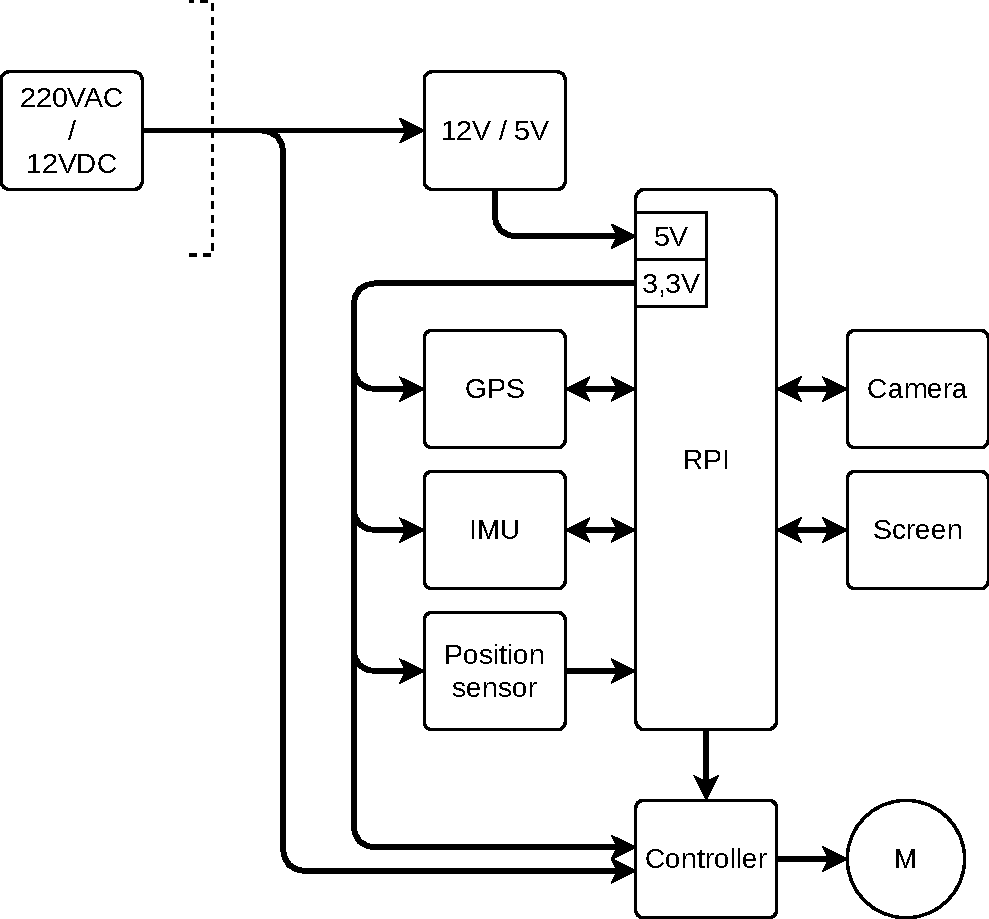
\includegraphics[width=0.7\linewidth]{\figures/sch_hardware.pdf}
    \decoRule
    \caption[
    Schéma structurel de premier niveau du télescope]{
    Schéma structurel de premier niveau du télescope}
    \label{fig:Schéma structurel de premier niveau du télescope}
    \end{figure}

\section{Conception du circuit}

\begin{figure}[H]
    \centering
    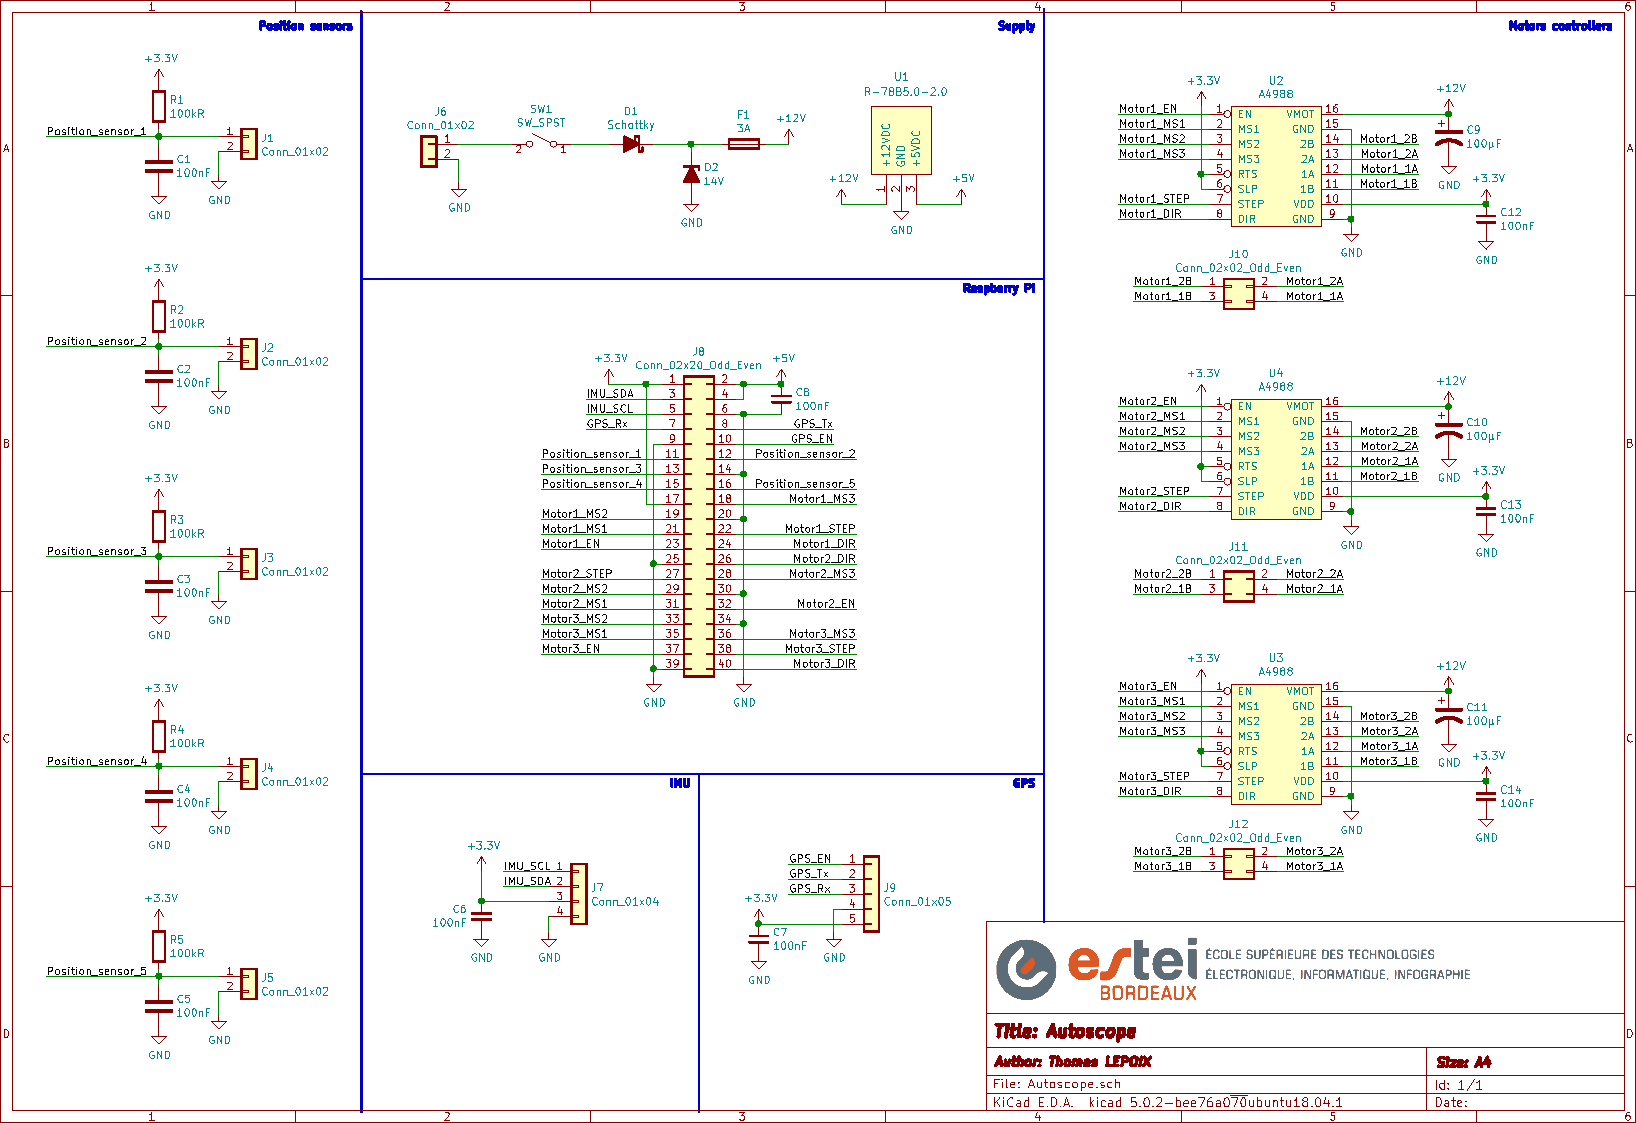
\includegraphics[width=1\linewidth]{\figures/kicad_sch2.pdf}
    \decoRule
    \caption[
    Schéma structurel de la carte du télescope]{
    Schéma structurel de la carte du télescope}
    \label{fig:Schéma structurel de la carte du télescope}
    \end{figure}

\vspace{1cm}

Ce schéma ne présente pas de subtilité particulière, la plupart des composants étant des connecteurs.

\vspace{1cm}

L'alimentation est composée de~:
\begin{itemize}[label=$\bullet$]
	\item Un interrupteur d'allumage
	\item Une diode polarisante
	\item Une diode zener protégeant des surtensions
	\item Un fusible protégeant des surintensités
	\item Un convertisseur DC/DC intégré
	\end{itemize}

\vspace{1cm}

L'environnement des boutons poussoirs servant de capteurs de butée aux mouvements du télescope est le suivant~:

\begin{figure}[H]
    \centering
    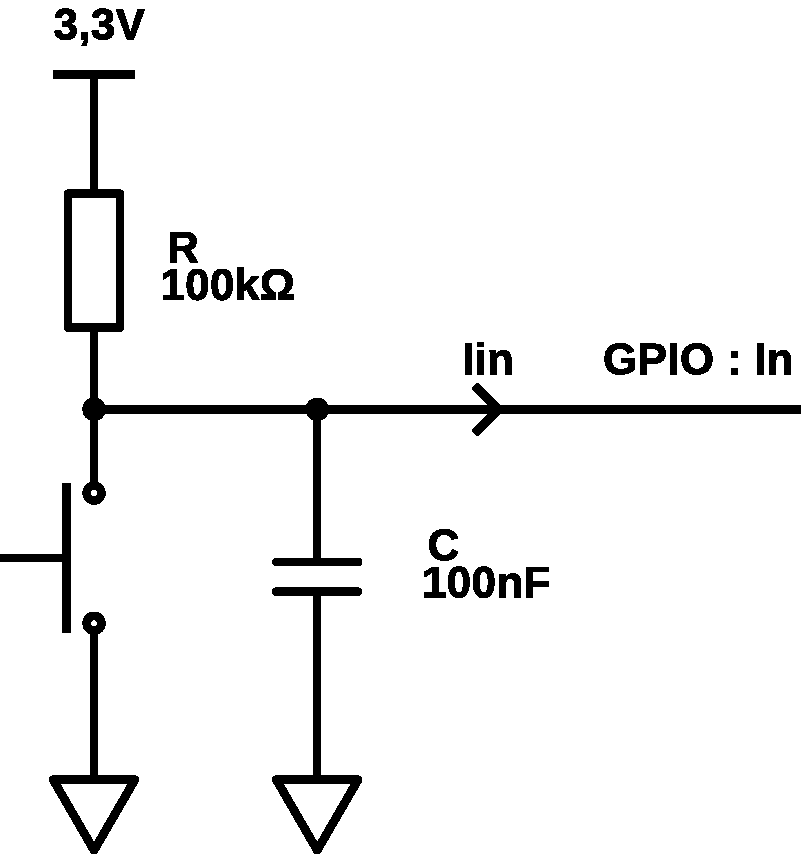
\includegraphics[width=0.3\linewidth]{\figures/sch_button.pdf}
    \decoRule
    \caption[
    Schéma de l'environnement des capteurs de butée]{
    Schéma de l'environnement des capteurs de butée}
    \label{fig:Schéma de l'environnement des capteurs de butée}
    \end{figure}

\vspace{1cm}

La valeur élevée des résistances de pullup $100k\Omega$ a pour but de réduire au maximum le courant consommé lors de l'appui, à $33\mu A$. Le courant prélevé par l'entrée GPIO de la Raspberry Pi est de l'ordre de $0,5\mu A$.

Les condensateurs de $100nF$ permettent de filtrer les parasites générés par les rebonds propres aux boutons ainsi que les perturbations électromagnétiques.

\section{Contraintes de design}

\subsection{Contraintes électromagnétiques}

La première contrainte vient de la proximité du système électronique de deux moteurs, ceux-ci générant d'importantes perturbations électromagnétiques. Cela peut être particulièrement dérangeant pour le fonctionnement de la centrale inertielle et du GPS.

La solution la plus simple et efficace est de déporter ces deux modules le long de la structure du télescope.

%\vspace{1cm}

\subsection{Contraintes mécaniques}

Ensuite viennent les contraintes mécaniques de l'association de la carte à la Raspberry Pi.

\vspace{1cm}

Tout d'abord, l'emplacement du connecteur et des fixations sont à prendre en compte.

\begin{figure}[H]
    \centering
    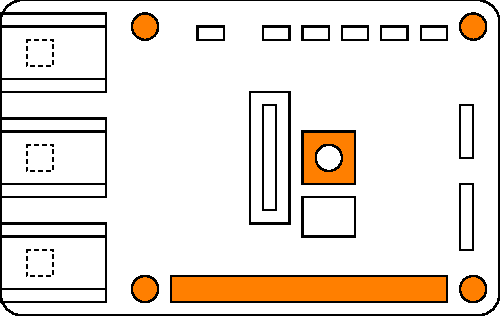
\includegraphics[width=0.5\linewidth]{\figures/sch_hard_1.pdf}
    \decoRule
    \caption[
    Schéma mécanique de la carte vue de dessus]{
    Schéma mécanique de la carte vue de dessus}
    \label{fig:Schéma mécanique de la carte vue de dessus}
    \end{figure}

\vspace{1cm}

Le connecteur d'alimentation, centré sur la carte, est un connecteur cylindrique comme ceux des ordinateurs portables. Le télescope étant amené à tourner sur lui même, ce connecteur devrait permettre le mouvement tout en empêchant le câble d'alimentation de s'emmêler ou de se détériorer.

\begin{figure}[H]
    \centering
    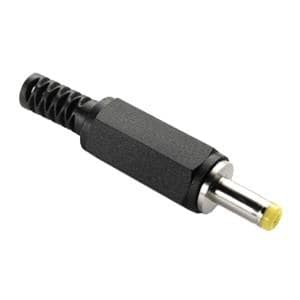
\includegraphics[height=0.3\linewidth]{\figures/photo_supply.jpg}
	\hspace{1cm}
    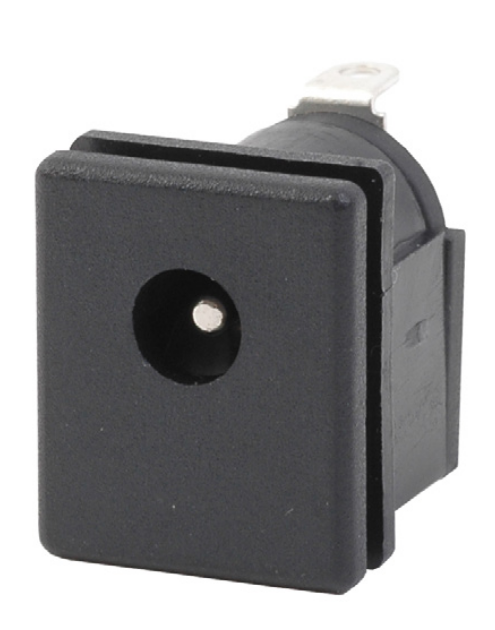
\includegraphics[height=0.3\linewidth]{\figures/photo_supply.png}
    \decoRule
    \caption[
    Connecteurs d'alimentation utilisés]{
    Connecteurs d'alimentation utilisés}
    \label{fig:Connecteurs d'alimentation utilisés}
    \end{figure}

\vspace{1cm}

Puis concernant la distance entre la carte et la Raspberry Pi, la hauteur des plus hauts éléments de la Raspberry Pi est à prendre en compte. Ainsi que la hauteur de certains condensateurs de la carte, ne pouvant donc être placés n'importe où.

\begin{figure}[H]
    \centering
    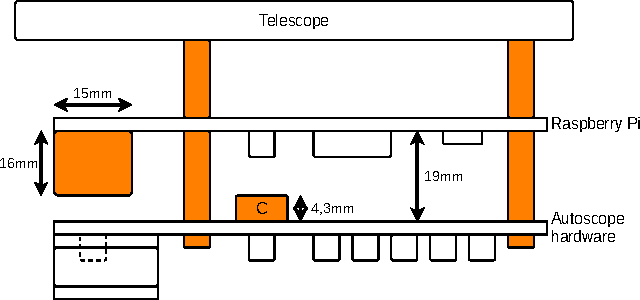
\includegraphics[height=0.23\linewidth]{\figures/sch_hard_2.pdf}
%	\hspace{1cm}
    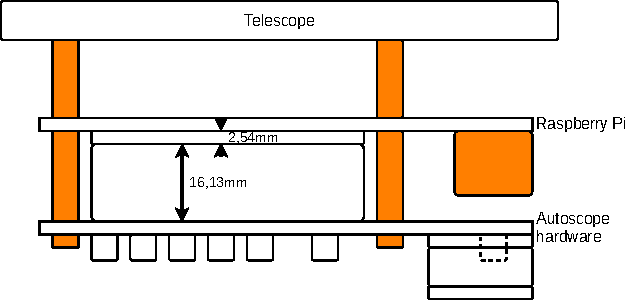
\includegraphics[height=0.23\linewidth]{\figures/sch_hard_3.pdf}
    \decoRule
    \caption[
    Schéma mécanique de la carte vue de profil]{
    Schéma mécanique de la carte vue de profil}
    \label{fig:Schéma mécanique de la carte vue de profil}
    \end{figure}

\vspace{1cm}

Il faudra de plus utiliser un connecteur particulièrement haut ($16,13mm$) pour relier la carte à la Raspberry Pi.

\begin{figure}[H]
    \centering
    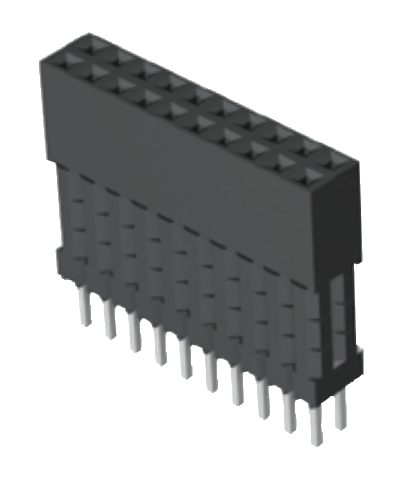
\includegraphics[width=0.3\linewidth]{\figures/photo_header.png}
    \decoRule
    \caption[
    Type de header utilisé]{
    Type de header utilisé}
    \label{fig:Type de header utilisé}
    \end{figure}

\section{Routage de la carte}

Le routage de la carte n'est pas terminé, voici un aperçu de son avancement actuel~:

\begin{figure}[H]
    \centering
    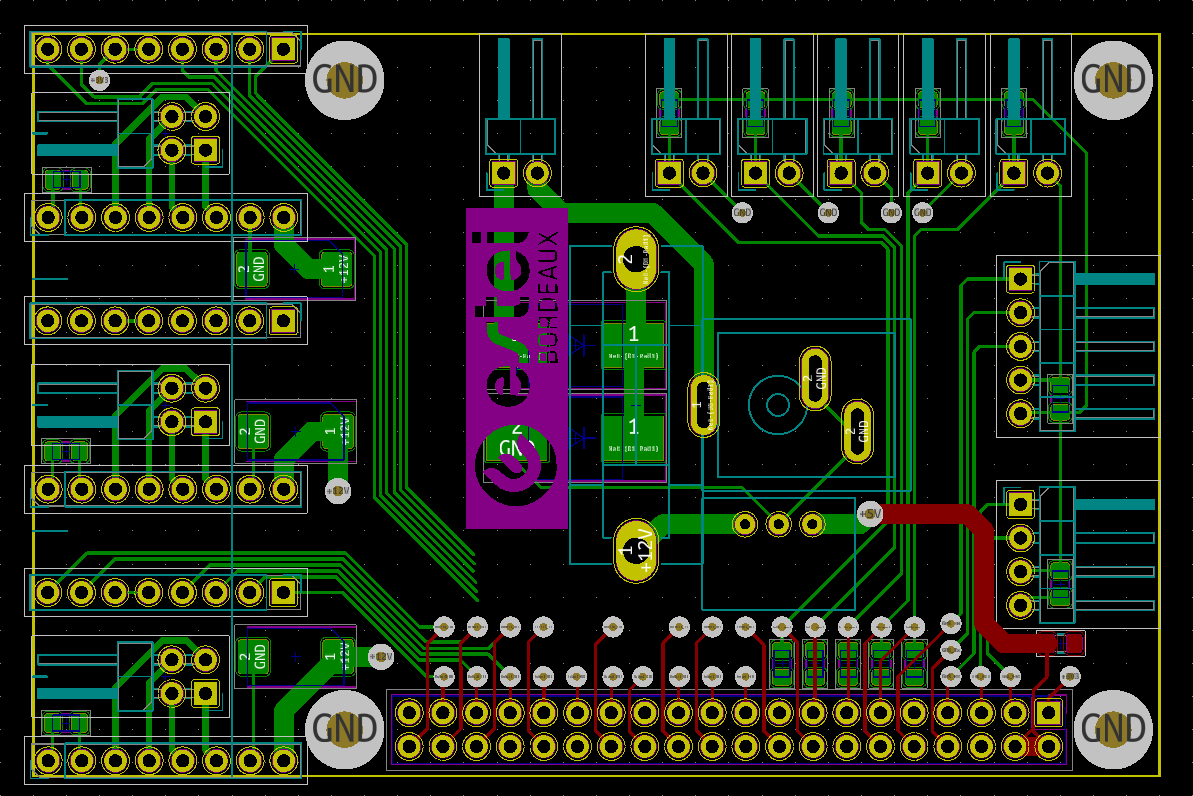
\includegraphics[width=0.7\linewidth]{\figures/kicad_pcb.png}
    \decoRule
    \caption[
    Aperçu du routage en cours]{
    Aperçu du routage en cours}
    \label{fig:Aperçu du routage en cours}
    \end{figure}

